% !TEX TS-program = xelatex
% !BIB TS-program = bibtex
\documentclass[12pt,letterpaper]{article}
\usepackage{style/dsc180reportstyle} % import 
\usepackage{footmisc}
% dsc180reportstyle.sty

%%%%%%%%%%%%%%%%%%%%%%%%%%%%%%%%%%%%%%%%%%%%%%%%%%%%%%%%
%%%% Title and Authors
%%%%%%%%%%%%%%%%%%%%%%%%%%%%%%%%%%%%%%%%%%%%%%%%%%%%%%%%

\title{DSC Capstone | Hardware Accelerators}

\author{Owen Shi \\
  {\tt a4shi@ucsd.edu} \\\And
  Pranav Kumarsubha \\
  {\tt pkumarsubha@ucsd.edu} \\\And
  Brendan Kuang \\
  {\tt blkuang@ucsd.edu} \\\And
  Edgar Guzman \\
  {\tt eiguzman@ucsd.edu} \\\And
  Idhant Kumar \\
  {\tt ikumar@ucsd.edu} \\\And
  Brandon Chiou \\
  {\tt 	brchiou@ucsd.edu} \\\And
  Rajesh Gupta \\
  {\tt rgupta@ucsd.edu} \\}

\begin{document}
\maketitle

%%%%%%%%%%%%%%%%%%%%%%%%%%%%%%%%%%%%%%%%%%%%%%%%%%%%%%%%
%%%% Abstract and Links
%%%%%%%%%%%%%%%%%%%%%%%%%%%%%%%%%%%%%%%%%%%%%%%%%%%%%%%%

\begin{abstract}
    We investigate the integration of an approximate linear-complexity multiplication algorithm (L-Mul) for neural network inference, evaluating its accuracy and performance characteristics across multiple software implementations and neural network architectures. We developed comprehensive software implementations of L-Mul in Python, NumPy, and PyTorch, enabling both scalar and matrix-level operations for testing and integration. Our evaluation demonstrates that L-Mul maintains accuracy within 1\% of standard floating-point multiplication across multilayer perceptron (MLP), convolutional neural network (CNN), and long short-term memory (LSTM) architectures, with 96.6\% prediction agreement in LSTM experiments. We implemented a Verilog hardware design and conducted simulation-based performance analysis, revealing that software optimizations cannot compete with native BLAS-optimized operations, highlighting the need for hardware acceleration to realize L-Mul's theoretical efficiency advantages. Our synthesis results demonstrate a 66.8\% area reduction compared to standard IEEE multipliers, validating L-Mul's hardware efficiency claims. Our results suggest that L-Mul can serve as an energy-efficient alternative to traditional floating-point multiplication for neural network inference, with future work focusing on theoretical performance analysis using Amdahl's law, evaluation of Transformer architectures, and comprehensive analysis of implementation costs and system integration challenges.
\end{abstract}

\begin{center}
Code: \url{https://github.com/oowenn/LMUL-Hardware-Acceleration}
\end{center}

\maketoc
\clearpage

%%%%%%%%%%%%%%%%%%%%%%%%%%%%%%%%%%%%%%%%%%%%%%%%%%%%%%%%
%%%% Main Contents
%%%%%%%%%%%%%%%%%%%%%%%%%%%%%%%%%%%%%%%%%%%%%%%%%%%%%%%%

\section{Introduction}

As artificial intelligence systems continue to scale in complexity and computational demand, speed and energy efficiency has emerged as a critical constraint. Neural networks require billions of floating-point operations during inference, with traditional IEEE 754 multiplication incurring substantial computational overhead. The \textit{L-Mul} (Linear-complexity Multiplication) algorithm presents an alternative approach: replacing expensive mantissa multiplication with addition-based operations to achieve $O(m)$ time complexity compared to the $O(m^2)$ time complexity of IEEE.

This report presents our implementation and validation of the L-Mul algorithm for neural network inference. We focus specifically on BFloat16 (BF16) arithmetic, a 16-bit floating-point format widely adopted in machine learning due to its compatibility with FP32 exponents while requiring only half the storage. Building upon theoretical foundations established by prior work, we address three primary objectives. First, we develop a functionally correct Verilog implementation of L-Mul for BF16 arithmetic along with test bench simulations. Next, we implement and test software implementations of L-Mul via Python, NumPy, and PyTorch. Finally, we implement and observe the accuracy tradeoffs of L-Mul in MLPs, CNNs, and LSTMs on classification tasks such as MNIST and Fashion MNIST.

\section{Methods}

\subsection{Standard BFloat16 Multiplication}

\label{subsec:standard_bf16}

Before discussing the L-Mul approximation, we first establish how standard BFloat16 multiplication works. BFloat16 (BF16) is a 16-bit floating-point format consisting of 1 sign bit, 8 exponent bits, and 7 mantissa bits. This format is particularly popular in machine learning due to its compatibility with single-precision (FP32) exponents while requiring only half the storage.

A BF16 number $x$ represents the value:

\begin{equation}
x = (-1)^s \times 2^{e - 127} \times (1.m)
\label{eq:bf16_representation}
\end{equation}

where $s$ is the sign bit, $e$ is the 8-bit exponent, $m$ represents the 7-bit mantissa, and 127 is the bias.

Standard BF16 multiplication follows the IEEE 754 approach: the signs are XORed, the exponents are added (with bias correction), and the mantissas are multiplied. This mantissa multiplication is the expensive part—it requires a hardware multiplier and subsequent normalization logic to handle carries. For neural network inference where millions of multiplications occur, this computational cost adds up quickly in terms of both latency and power consumption.

\subsection{LMUL Algorithm}

\label{subsec:lmul_algorithm}

The L-Mul algorithm takes a different approach. Instead of treating the exponent and mantissa as separate entities, it exploits a clever observation: if we treat the combined exponent-mantissa field as a single fixed-point number, multiplication can be approximated by simple addition. This works because logarithms transform multiplication into addition, and the floating-point exponent already represents a logarithmic quantity.

\paragraph{Algorithm Overview.}

Given two BF16 operands $a$ and $b$, L-Mul works by adding their exponent-mantissa fields directly. Here's how it breaks down:

\textbf{Step 1: Extract the fields.} We pull out the components from each 16-bit operand:

\begin{align}
a_{sign} &= a[15], \quad b_{sign} = b[15] \\
a_{field} &= a[14:0], \quad b_{field} = b[14:0]
\end{align}

The $field$ values contain the concatenated exponent and mantissa bits, which we'll treat as a single 15-bit integer.

\textbf{Step 2: Handle edge cases.} If either input is zero or subnormal (indicated by a zero exponent), we immediately return zero. This keeps the algorithm simple and handles the most common edge case:

\begin{equation}
\text{if } a_{exp} = 0 \text{ or } b_{exp} = 0 \text{, return } 0
\end{equation}

\textbf{Step 3: Add the fields.} We add the two fields together, but we need to correct for the fact that adding exponents naturally doubles the bias:

\begin{equation}
\text{sum}_{full} = a_{field} + b_{field} + \text{OFFSET}_{MOD}
\label{eq:lmul_addition}
\end{equation}

The offset term compensates for this doubled bias:

\begin{equation}
\text{OFFSET}_{MOD} = ((2^{15}) - (127 \ll 7)) \text{ AND } 0x7FFF = 0x4080
\end{equation}

We use 17 bits for the sum to capture potential overflow.

\textbf{Step 4: Check for overflow or underflow.} The top two bits of our 17-bit sum tell us what happened:

\begin{equation}
\text{carry}_2 = \text{sum}_{full}[16:15]
\end{equation}

These bits give us three cases:

\begin{itemize}
    \item $00_2$: The result underflowed—return zero
    \item $01_2$: Normal result—use the lower 15 bits
    \item $1x_2$: The result overflowed—saturate to maximum value ($0x7FFF$)
\end{itemize}

\textbf{Step 5: Calculate the sign.} This follows standard multiplication rules—XOR the input signs, but force the result to positive zero if the magnitude is zero:

\begin{equation}
s_{result} = \begin{cases}
0 & \text{if field} = 0 \\
a_{sign} \oplus b_{sign} & \text{otherwise}
\end{cases}
\end{equation}

\textbf{Step 6: Pack the result.} Finally, we combine the sign bit with the selected field value:

\begin{equation}
\text{result} = (s_{result} \ll 15) \text{ OR } \text{field}_{sel}
\end{equation}

\paragraph{Why This Works.}

The key insight is that the exponent field already represents a logarithm (base 2), and the mantissa can be approximated as part of this logarithmic representation. When we add these combined fields, we're essentially performing multiplication in log space. The approximation comes from treating the mantissa bits as part of a continuous logarithmic scale rather than as a separate fractional multiplier. For neural network inference, this approximation is remarkably accurate—accurate enough that we see virtually no loss in classification accuracy, as we'll show in the results.

\subsection{Development Environment and Docker Configuration}

Docker was used for containerization to ensure consistent package reliability across different machines. Using the relevant files, a VS Code pipeline was developed to automate the installation of necessary Python and Verilog dependencies, while ensuring compatibility, as well as relevant VS Code extensions such as Python and Jupyter.

\subsection{Verilog Simulation}

\label{subsec:simulation_infrastructure}

To validate our LMUL hardware design and enable integration with machine learning workloads, we developed a simulation pipeline that bridges Verilog hardware descriptions with Python-based testing and neural network frameworks. This infrastructure allows us to verify correctness, measure performance characteristics, and ultimately test LMUL on real ML tasks without requiring physical hardware.

\paragraph{Simulation Approach.}

We use Icarus Verilog (iverilog), an open-source Verilog simulator, to compile and execute our hardware descriptions. The simulation flow works as follows: our Verilog modules are compiled into an executable simulation model, which we then run using the \texttt{vvp} (Verilog VVP) runtime. This generates cycle-accurate behavior that matches what the actual hardware would do, including all timing, handshaking protocols, and pipeline stages.

\paragraph{Batch Testing Architecture.}

Rather than spawning a new simulation process for every single multiplication (which would be prohibitively slow), we developed a batch testing system. Our \texttt{BatchLMULTester} class generates a complete Verilog testbench that includes:

\begin{itemize}
    \item Arrays of pre-loaded test input pairs ($a$, $b$)
    \item Clock generation and reset logic
    \item Ready/valid handshaking to properly interface with our LMUL module's pipeline
    \item Result capture logic that stores outputs as they become available
    \item Automatic result printing for parsing by Python
\end{itemize}

This approach means we compile and run the simulator once per batch, rather than once per operation. For testing 1000 multiplications, this reduces overhead from roughly 50 seconds to about 30 milliseconds, a speedup of over 1500x compared to naive per-operation simulation.

\paragraph{Parallelized Testing Architecture.}

To further enhance our simulation performance and diagnostic capabilities, we explored a parallelized approach by instantiating multiple Designs Under Test (DUT) to operate on multiple numbers in one clock cycle. This yielded minimal speed gains due to the serial nature of our DUT instantiation and the single-threaded execution of Icarus Verilog and vvp. We shifted our simulation environment from Icarus Verilog to Vivado, a dedicated FPGA development tool, which enables detailed waveform generation for precise bottleneck identification and correctness verification. Additionally, we optimized input signals by removing unnecessary handshaking logic, reducing input signal latency from 20ns to 10ns and effectively halving the simulation runtime associated with positive clock edges.

\subsection{Hardware Synthesis Methodology}

\label{subsec:synthesis_methodology}

While our simulation work (Section~\ref{subsec:simulation_infrastructure}) validated the functional correctness of our L-Mul hardware design, synthesis provides concrete hardware metrics that quantify the efficiency advantages. To validate the hardware efficiency claims of L-Mul and obtain quantitative metrics for comparison with standard IEEE BF16 multiplication, we synthesized both designs using industry-standard EDA tools. This synthesis process converts our Verilog RTL descriptions into gate-level netlists mapped to a standard cell library, enabling quantitative comparison of area and architectural characteristics.

\paragraph{Synthesis Flow.}

We used Yosys 0.9, an open-source synthesis tool, to perform technology mapping of both multiplier designs to the Nangate 45nm Open Cell Library. The synthesis flow for each design followed a standard sequence: (1) reading the Verilog RTL and standard cell library, (2) hierarchy processing and optimization, (3) finite state machine optimization, (4) memory optimization, (5) flattening for technology mapping, (6) flip-flop mapping to library cells, (7) combinational logic mapping using ABC with a 1.0 ns target clock period, and (8) final optimization and cleanup. This process generated gate-level netlists where each logic operation is implemented using standard cells from the Nangate library, providing concrete area and cell count metrics for comparison.

\paragraph{Design Wrappers.}

To ensure fair comparison, we created synthesis-specific wrapper modules that isolate the core multiplier logic from testbench code. The L-Mul wrapper instantiates our \texttt{lmul\_bf16} module, while the IEEE BF16 wrapper instantiates a standard IEEE-754 BF16 multiplier implementation that performs full mantissa multiplication. Both wrappers maintain identical interfaces with ready/valid handshaking protocols, ensuring equivalent control logic overhead in the comparison.

\paragraph{Technology Library.}

The Nangate 45nm Open Cell Library provides a comprehensive set of standard cells including basic logic gates (AND, OR, XOR, NAND, NOR), complex gates (AOI, OAI), flip-flops, and specialized cells. This library is widely used in academic research and provides realistic area and timing characteristics for 45nm CMOS technology. All area measurements are reported in library-specific area units, which represent the physical silicon area required for each standard cell.

\subsection{Software Testing}

To support comprehensive validation and performance analysis of LMUL across different computational contexts, we developed multiple software implementations targeting distinct use cases. These implementations enable us to verify correctness and benchmark performance characteristics.

\paragraph{Scalar Implementations and Comparisons.}

For element-wise multiplication operations, we implemented scalar LMUL versions across multiple frameworks. Our pure Python scalar implementation processes individual BF16 operand pairs and serves as our primary reference for validation, providing a fast and transparent way to generate expected results without the overhead of hardware simulation. The Python version follows the exact same algorithm as our Verilog implementation, ensuring bit-exact matches for verification. For efficient batch processing, we developed vectorized NumPy and PyTorch implementations that operate on entire arrays of BF16 values simultaneously, leveraging optimized array operations and SIMD capabilities to process thousands of element-wise multiplications in parallel. These scalar implementations are used in our speed and accuracy testing frameworks to compare LMUL performance and accuracy against standard floating-point multiplication across different input ranges and batch sizes, enabling us to understand the performance characteristics and numerical behavior of LMUL at the fundamental operation level.

\paragraph{Matrix Multiplication Implementations and Comparisons.}

For matrix-level operations, we implemented LMUL-based matrix multiplication functions in both NumPy and PyTorch that perform full matrix multiplications using LMUL for the underlying element-wise products. These implementations broadcast input matrices to compute all pairwise LMUL products, then sum along the appropriate dimensions to produce matrix multiplication results. The NumPy implementation enables direct comparison with standard BLAS-optimized matrix multiplication, while the PyTorch version integrates with neural network frameworks and includes a custom \texttt{torch.autograd.Function} that enables automatic differentiation during training. Our matrix multiplication implementations are evaluated in dedicated speed and accuracy testing frameworks that compare LMUL-based matrix operations against standard NumPy and PyTorch matrix multiplication across various matrix sizes, revealing how the approximate nature of LMUL propagates through matrix operations and providing performance benchmarks for potential neural network integration scenarios.

\subsection{MLP–L-Mul Integration}

\label{subsec:mlp_lmul}

To investigate the integration of approximate arithmetic within neural networks, we implemented a modified multilayer perceptron (MLP) in PyTorch capable of operating under both conventional and L-Mul modes. The objective was to directly substitute the standard floating-point multiply operation in the forward pass with an approximate function that more closely resembles a hardware-efficient arithmetic primitive.

\paragraph{Model Architecture.}

The MLP architecture consists of two fully connected layers with ReLU activations, followed by a log-softmax output layer. The first layer maps a flattened $28\times 28$ input image to a 128-dimensional hidden representation, while the second projects to the 10 output classes corresponding to the MNIST digits. 

\paragraph{Vectorized Implementation.}

For efficiency, a custom function \texttt{lmul\_linear} was implemented to perform the equivalent of a dense linear transformation using L-Mul arithmetic. Given an input tensor $x \in \mathbb{R}^{B \times I}$ and a weight matrix $W \in \mathbb{R}^{O \times I}$, the computation proceeds as

\begin{equation}
Y_{b,o} = \sum_{i=1}^{I} \text{L-Mul}(x_{b,i}, W_{o,i}) + b_o
\end{equation}

where $b$ denotes the batch dimension. Broadcasting and tensor expansion were used to apply L-Mul elementwise over all input–weight pairs, followed by summation across input features.

\paragraph{Training and Evaluation Procedure.}

The model was first trained for both two and five epochs on the MNIST training set using standard floating-point arithmetic and the Adam optimizer. After training, the learned weights were evaluated under the L-Mul mode using the same architecture and parameter values. This allowed direct comparison between true multiplication and its L-Mul approximation under identical learned representations. All experiments were conducted on CPU using PyTorch's built-in automatic differentiation and tensor operations.

\subsection{LSTM–L-Mul Integration}

To test L-Mul's approximation cost among other neural networks, we implemented a Long-Short Term Memory (LSTM) in PyTorch capable of operating under both conventional and L-Mul multiplication. Like the MLP, the objective is to directly substitute the standard floating-point multiply operation in the forward pass with an approximate function (L-Mul). 

\paragraph{Model Architecture.}

For each timestep in a sequence, the input embedding $x_t$ is concatenated with the previous hidden state $h_{t-1}$ and passed through linear transformations to compute the LSTM gates: input ($i_t$), forget ($f_t$), cell candidate ($g_t$), and output ($o_t$). The cell state $c_t$ and hidden state $h_t$ are then updated according to the standard LSTM equations:

\begin{equation}    
c_t = f_t \odot c_{t-1} + i_t \odot g_t, \quad
h_t = o_t \odot \tanh(c_t)
\end{equation}


For sequence classification, the final hidden state $h_T$ is used as input to a linear layer to produce logits for the output classes. A token is sampled from these logits, and its embedding is used as the input for the next timestep. The hidden and cell states carry over, providing context, while the logits themselves are only used for sampling and not fed directly back into the model. For language modeling, each timestep's hidden state can be used to predict the next token, and generation continues recursively until an end-of-sequence token or a maximum length is reached.

\paragraph{PyTorch L-Mul Implementation}  

Considering that the LSTM is significantly more computationally intensive than the MLP layer, a specialized L-Mul algorithm was implemented to optimize runtime and allow PyTorch compilation. The algorithm simulates bfloat16 multiplication within float32 tensors by extracting the sign and field bits of each input, performing field addition with bias correction, and handling underflow and overflow conditions explicitly. The resulting bits are then repacked into a float32 tensor, with a small heuristic bitshift correction added to improve accuracy for LSTM operations, where multiplication errors accumulate rapidly. Finally, zeros and subnormal values are explicitly managed to maintain numerical stability. 

\paragraph{Training and Evaluation Procedure.}

The model was first trained for three epochs across 5 seeds on the FashionMNIST, KMNIST, SeqMNIST datasets using standard floating-point arithmetic and the Adam optimizer. As in the MLP Layer methodology section, after training, the learned weights were evaluated under the L-Mul mode using the same architecture and parameter values against floating-point multiplication.

\subsection{CNN–L-Mul Integration}
\label{subsec:cnn_lmul}

To evaluate L-Mul in a convolutional architecture, we implemented a simple convolutional neural network (CNN) capable of operating under both conventional and L-Mul multiplication modes. The objective was to observe the effect of L-Mul on a model that relies heavily on convolutional layers, maintaining the same architecture and training process while only changing the multiplication operator during inference.

\paragraph{Model Architecture.}

The CNN consists of two convolutional layers followed by two fully connected layers. The first convolution produces 32 feature maps and the second produces 64 feature maps. After each convolution, we apply a ReLU activation followed by max pooling to reduce spatial size. The output is flattened and passed through a linear layer with 128 units, followed by a final layer that returns 10 class scores.

\paragraph{Using L-Mul Inside Convolutions.}

To use L-Mul in this setting, we created a version of the convolution calculation where every multiplication between the input and kernel weight is replaced by L-Mul. We used broadcasting so that the operator applies across all spatial positions and channels simultaneously. The summation part of the convolution remains unchanged, allowing us to keep the overall structure of the operation while changing only the arithmetic.

\paragraph{Training and Evaluation Procedure.}

The model was trained normally using floating-point arithmetic on MNIST. After training, we ran two evaluations: the first used standard multiplication and the second used L-Mul for all multiplications in both the convolutional and linear layers. Since everything else in the model stayed the same, any difference in accuracy comes from the arithmetic change alone.

\section{Results}

\subsection{Numerical Accuracy Evaluation}

We evaluated the accuracy of LMUL implementations at both the scalar (element-wise) and matrix multiplication levels, comparing them against standard floating-point arithmetic and verifying consistency across different software implementations.

\paragraph{Scalar Accuracy Evaluation.}

For element-wise multiplication operations, we compared multiple LMUL implementations against standard floating-point multiplication. Our evaluation includes Python scalar LMUL, NumPy vectorized LMUL, PyTorch vectorized LMUL, and Verilog hardware simulation, all tested against standard IEEE 32-bit floating-point multiplication. For each test configuration, we generated $N = 10,000$ randomly sampled operand pairs, with each operand drawn uniformly from the range [-10,000, +10,000]. The inputs were evaluated by all multiplication methods, and the average absolute error was normalized by the numerical range of the test dataset to yield a percentage error metric.

The results demonstrate that all LMUL implementations produce consistent results, with the Verilog hardware simulation matching the Python LMUL emulator exactly. When compared to standard floating-point multiplication, LMUL exhibits a bounded and predictable precision loss consistent with the reduced precision of the BF16-style format used internally. These results indicate that LMUL preserves correctness relative to its software specification while introducing precision loss that is small enough to support downstream inference tasks.

\begin{figure}[h]
    \centering
    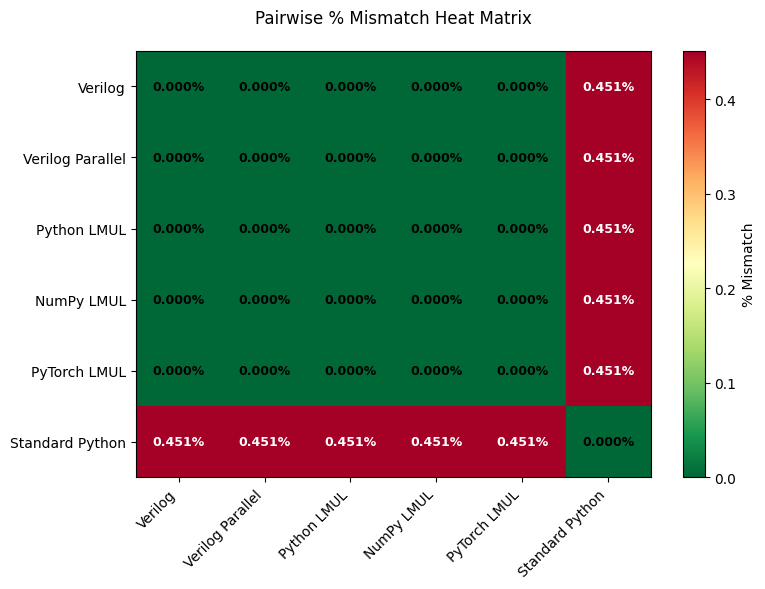
\includegraphics[width=0.9\linewidth]{figure/scalar_accuracy.png}
    \caption{Accuracy comparison of scalar LMUL implementations against standard floating-point multiplication.}
    \label{fig:scalar_accuracy}
\end{figure}

\paragraph{Matrix Multiplication Accuracy Evaluation.}

For matrix-level operations, we evaluated LMUL-based matrix multiplication against standard NumPy and PyTorch matrix multiplication implementations. We tested $N = 100$ randomly generated matrix pairs of size $20 \times 20$, with values drawn from uniform distributions. The evaluation compares NumPy standard matrix multiplication, PyTorch standard matrix multiplication, NumPy LMUL matrix multiplication, and PyTorch LMUL matrix multiplication, measuring pairwise percentage mismatch between implementations.

The results reveal how the approximate nature of LMUL propagates through matrix operations, showing the cumulative effect of element-wise approximation errors when aggregated across full matrix multiplications. This analysis provides insights into the numerical stability of LMUL for neural network applications where matrix operations are fundamental.

\begin{figure}[h]
    \centering
    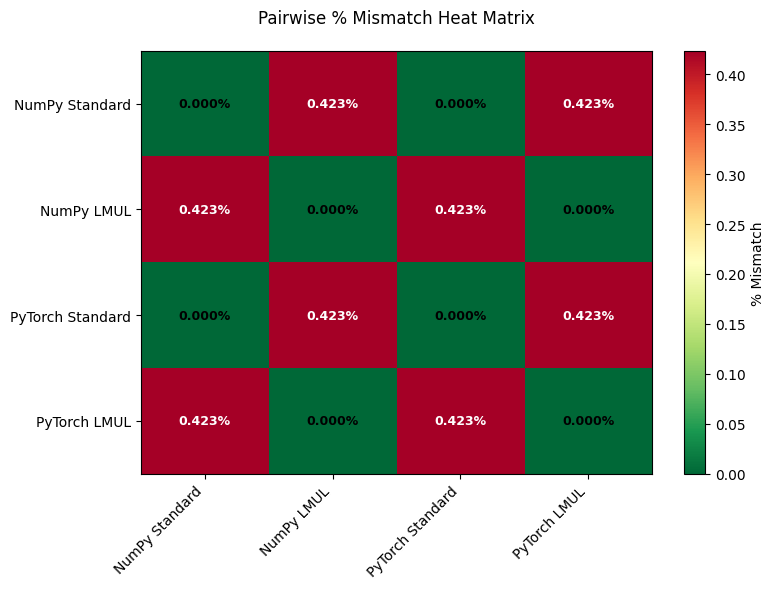
\includegraphics[width=0.9\linewidth]{figure/matrix_accuracy.png}
    \caption{Pairwise accuracy comparison heat matrix for matrix multiplication implementations.}
    \label{fig:matrix_accuracy}
\end{figure}

\subsection{Execution Speed}

We benchmarked the performance of LMUL implementations at both scalar and matrix multiplication levels, comparing them against standard implementations across various batch sizes and matrix dimensions.

\paragraph{Scalar Multiplication Speed.}

We benchmarked multiple multiplication backends for element-wise operations across batch sizes ranging from $10^1$ to $10^5$ operations. The evaluation includes standard Python \texttt{float32} multiplication, NumPy vectorized multiplication, PyTorch vectorized multiplication, Python scalar LMUL, NumPy vectorized LMUL, PyTorch vectorized LMUL, Verilog LMUL hardware simulation, and parallelized Verilog simulation with 4 DUTs. The measured quantity is the average time per multiplication after removing initialization overhead.

As shown in Figure~\ref{fig:scalar_speed}, NumPy achieves the lowest latency due to optimized vectorized execution, reaching sub-nanosecond performance for large batches. Standard Python and PyTorch multiplications scale well as loop overhead amortizes. The LMUL hardware simulation path incurs larger per-call overhead from Verilog simulation, but its time per operation decreases with batch size. This reflects simulator cost rather than hardware speed---a synthesized implementation would operate at clock-cycle scale. The Python LMUL model is slower due to explicit bit-level emulation, while vectorized NumPy and PyTorch LMUL implementations provide intermediate performance.

\begin{figure}[h]
    \centering
    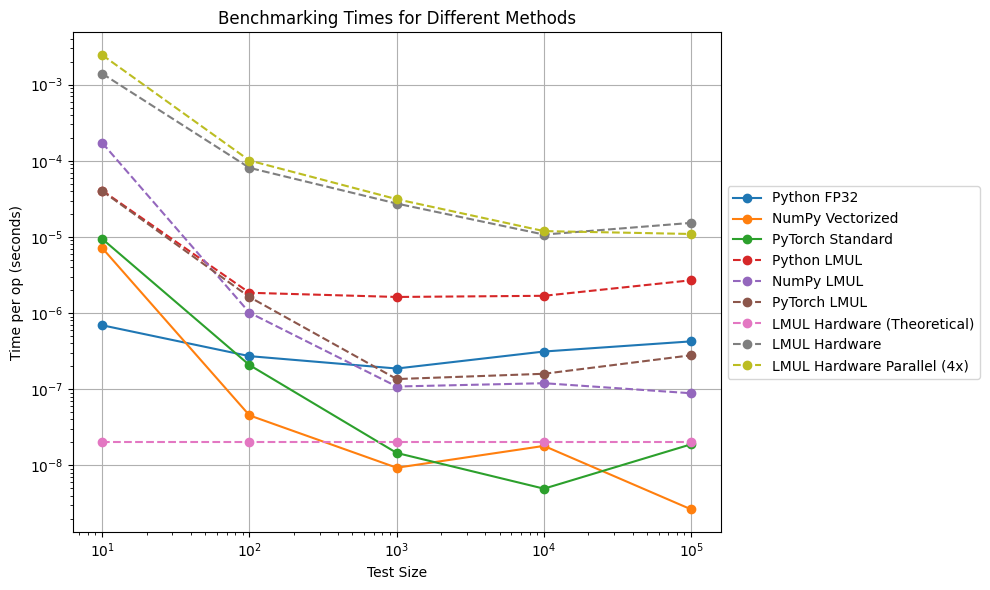
\includegraphics[width=\linewidth]{figure/scalar_speed.png}
    \caption{Average time per scalar multiplication (log--log scale) for multiple implementations over increasing batch sizes.}
    \label{fig:scalar_speed}
\end{figure}

\paragraph{Matrix Multiplication Speed.}

We benchmarked matrix multiplication performance for standard and LMUL-based implementations across matrix sizes ranging from $10 \times 10$ to $200 \times 200$. The evaluation compares NumPy standard matrix multiplication, PyTorch standard matrix multiplication, NumPy LMUL matrix multiplication, and PyTorch LMUL matrix multiplication. Performance is measured as time per operation normalized by matrix size ($n^3$ operations for $n \times n$ matrices).

As shown in Figure~\ref{fig:matrix_speed}, standard NumPy and PyTorch implementations leverage optimized BLAS routines for high performance. LMUL-based matrix multiplication implementations show different performance characteristics due to the overhead of BF16 conversion and element-wise LMUL operations, though they provide the approximate arithmetic needed for neural network inference scenarios. The results demonstrate the performance trade-offs when using approximate arithmetic for matrix operations in software implementations.

\begin{figure}[h]
    \centering
    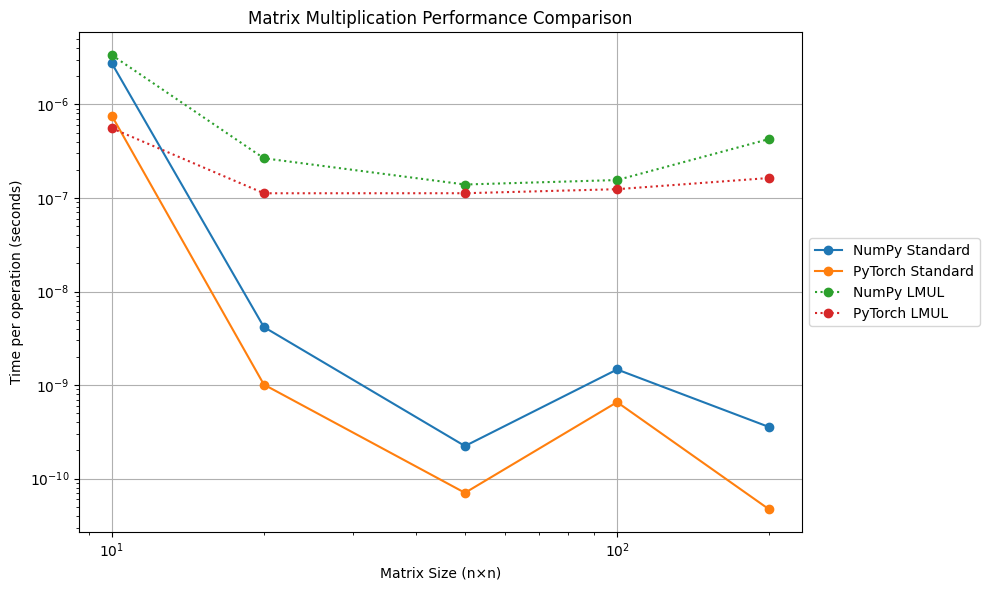
\includegraphics[width=\linewidth]{figure/matrix_speed.png}
    \caption{Time per operation for matrix multiplication implementations across different matrix sizes (log--log scale).}
    \label{fig:matrix_speed}
\end{figure}

\subsection{MLP–L-Mul Integration Results}

After training the baseline multilayer perceptron (MLP) for five epochs on the MNIST dataset using standard floating-point arithmetic, the model achieved a test accuracy of 97.02\%. The same trained weights were subsequently evaluated using the L-Mul arithmetic mode, in which all elementwise multiplications within the linear layers were replaced by the approximate L-Mul operator as described in Section~\ref{subsec:mlp_lmul}. The resulting test accuracy under L-Mul computation was 97.01\%.

This outcome supports the hypothesis that approximate arithmetic primitives such as L-Mul can be integrated into neural inference pipelines without sacrificing predictive accuracy, provided that proper magnitude calibration is applied. The finding also suggests that hardware implementations based on L-Mul may yield reductions in power consumption or silicon area without compromising functional correctness at the algorithmic level.

\subsection{LSTM L-Mul Integration Results}

We evaluated the impact of replacing standard FP32 multiplication with the L-Mul operator inside the LSTM cell across FashionMNIST, KMNIST, and SeqMNIST. For each configuration, five runs were performed to estimate mean accuracy and variance.

\begin{figure}[h!]
    \centering
    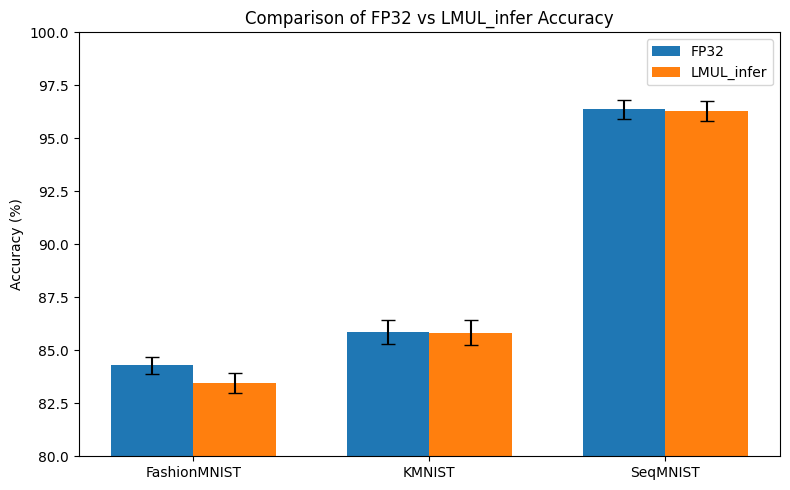
\includegraphics[width=0.9\linewidth]{figure/LSTMInfer.png}
    \caption{Comparison of FP32 vs.\ L-Mul inference accuracy across datasets. Error bars denote standard deviation over five runs.}
    \label{fig:lstm_infer_bar}
\end{figure}

As shown in Figure~\ref{fig:lstm_infer_bar}, across all datasets, L-Mul closely matches FP32 performance.

Overall, L-Mul introduces less than a \(1\%\) accuracy change across all tasks. Furthermore, upon investigating the FashionMNIST predictions between L-Mul and floating point multiplication LSTMs, there is a 96.6\% agreement rate between the two models. This demonstrates that the operator remains an effective approximation with relatively low classification error within a recurrent architecture (LSTM) but non-negligible prediction disagreement where multiplicative approximation errors can accumulate.

\subsection{CNN–L-Mul Integration Results}

We evaluated the impact of replacing standard FP32 multiplication with the L-Mul operator in the CNN architecture described in Section~\ref{subsec:cnn_lmul}. Table~\ref{tab:cnn_results} presents the test accuracy results for both standard and L-Mul arithmetic modes.

\begin{table}[h]
\centering
\begin{tabular}{lcc}
\hline
\textbf{Dataset} & \textbf{Standard FP32} & \textbf{L-Mul} \\
\hline
MNIST & 98.30\% & 98.07\% \\
\hline
\end{tabular}
\caption{CNN test accuracy comparison between standard FP32 and L-Mul arithmetic on MNIST.}
\label{tab:cnn_results}
\end{table}

The results demonstrate that L-Mul maintains accuracy within 1\% of the standard floating-point baseline, with a difference of only 0.23 percentage points on MNIST. This small accuracy difference suggests that the convolutional structure helps smooth out the error introduced by the approximate operator, consistent with what we observed in the MLP and LSTM experiments. Across all three model architectures (MLP, LSTM, and CNN), L-Mul maintains accuracy within approximately 1\% of the floating-point baseline, demonstrating its robustness across diverse neural network architectures.

\subsection{Hardware Synthesis Comparison}

To quantify the hardware efficiency advantages of L-Mul, we synthesized both the L-Mul and IEEE BF16 multiplier designs using the methodology described in Section~\ref{subsec:synthesis_methodology}. This synthesis process converts our Verilog RTL descriptions into gate-level netlists, enabling quantitative comparison of area and architectural characteristics.

\paragraph{Area Metrics.}

Table~\ref{tab:synthesis_area} presents the area comparison between L-Mul and IEEE BF16 multipliers. The L-Mul design achieves a 66.8\% reduction in standard cell area compared to the IEEE multiplier, using 180.88 area units versus 545.03 area units. This represents a 3.01× reduction in silicon area, meaning that approximately three L-Mul units can fit in the same area as one IEEE multiplier. The cell count comparison shows a 63.0\% reduction, with L-Mul requiring 181 cells compared to 489 cells for the IEEE design.

\begin{table}[h]
\centering
\begin{tabular}{lccc}
\hline
\textbf{Metric} & \textbf{L-Mul} & \textbf{IEEE BF16} & \textbf{Improvement} \\
\hline
Standard Cell Area & 180.88 units & 545.03 units & 66.8\% reduction \\
Number of Cells & 181 & 489 & 63.0\% reduction \\
Area Ratio (L-Mul/IEEE) & 0.332 & 1.000 & 3.01× smaller \\
\hline
\end{tabular}
\caption{Area comparison between L-Mul and IEEE BF16 multipliers synthesized with Nangate 45nm library.}
\label{tab:synthesis_area}
\end{table}

\paragraph{Architectural Analysis.}

The cell type breakdown reveals the fundamental architectural difference between the two designs. The L-Mul implementation uses only basic logic gates (AND, OR, XOR, NAND, NOR) and adders—no multiplier cells are present. In contrast, the IEEE BF16 multiplier contains complex multiplier logic implemented as optimized gate networks to perform 8×8 bit mantissa multiplication. This architectural difference explains the area savings: L-Mul avoids the expensive multiplier hardware entirely, replacing it with simple addition operations. This finding connects to our software and neural network results, demonstrating that L-Mul maintains accuracy despite using simpler arithmetic operations.

\section{Discussion}
The results obtained from our experiments demonstrate that the L-Mul algorithm can serve as a highly efficient approximation to standard floating-point multiplication with minimal loss in numerical accuracy. Our evaluation across MLP, LSTM, and CNN architectures shows that L-Mul maintains accuracy within 1\% of standard floating-point implementations, suggesting neural networks tolerate small arithmetic errors well across diverse architectures. The 96.6\% prediction agreement rate observed in LSTM experiments demonstrates that while multiplicative approximation errors can accumulate in recurrent architectures, the overall impact remains bounded and acceptable for inference tasks. The CNN results further support this finding, showing that convolutional structures help smooth out approximation errors. This resilience suggests that strict IEEE-754 compliance is unnecessary for effective inference, enabling hardware designs that favor efficiency over precision through L-Mul or similar methods.

From a software optimization perspective, our thorough exploration of vectorized implementations in NumPy and PyTorch revealed that while LMUL can be efficiently implemented using array operations and broadcasting, these software implementations are unable to compete with native BLAS-optimized floating-point operations in terms of raw performance. The overhead of BF16 conversion, element-wise LMUL computation, and lack of hardware-accelerated routines result in slower execution compared to standard matrix multiplication. This performance gap highlights the importance of hardware acceleration for LMUL to realize its theoretical efficiency advantages.

From a hardware perspective, the implications are substantial. Traditional floating-point multiplication is among the most power and area intensive operations in digital accelerators. Our Verilog simulation work (Section~\ref{subsec:simulation_infrastructure}) validated functional correctness, ensuring that the hardware design produces the same results as our software implementations, but simulation does not provide hardware efficiency metrics. Our synthesis results (Section~\ref{subsec:synthesis_methodology}) provide the missing quantitative evidence: L-Mul achieves a 66.8\% reduction in standard cell area and a 63.0\% reduction in cell count compared to IEEE BF16 multiplication, confirming that substituting multiplication with primarily addition-based logic significantly reduces gate count and silicon area. These synthesis results demonstrate that L-Mul's theoretical advantages translate to actual hardware efficiency, complementing our software accuracy results to show both algorithmic correctness and hardware efficiency.

\paragraph{Future Work.}
Several important directions remain for future exploration. First, while actual chip integration may be costly, we can leverage our unit operation test results to measure theoretical performance gains in real neural network models. By applying Amdahl's law based on the percentage of compute time spent on matrix multiplication operations, we can estimate the overall speedup and efficiency improvements that L-Mul would provide in deployed systems. This theoretical analysis, combined with our synthesis results quantifying area advantages (66.8\% reduction), provides a practical framework for evaluating L-Mul's impact without requiring expensive physical hardware implementation.

Second, further exploration of LMUL integration in diverse ML pipelines is warranted. Our current evaluation covers MLPs, LSTMs, and CNNs, but testing on Transformer architectures and sequential token generators would provide broader validation of LMUL's applicability. Experiments on more complex tasks such as language modeling and large-scale vision tasks would help establish the boundaries of LMUL's effectiveness, particularly in layers with high sensitivity to numerical error (e.g., attention mechanisms or normalization layers).

Third, a comprehensive analysis of the costs and obstacles associated with implementing a LMUL hardware accelerator is needed. This includes evaluation of chip manufacturing costs, integration complexity with existing systems, operating system compatibility, and software stack requirements. Understanding these practical constraints is crucial for assessing the real-world viability of LMUL as an alternative to traditional floating-point arithmetic in commercial AI accelerators.

\section{Conclusion}

In our report, we focused on the integration of the L-Mul algorithm into neural network architectures to explore how arithmetic approximation can coexist with conventional neural network operations. Our results showcase the successful implementation of L-Mul across multiple software frameworks, hardware simulation for correctness validation, and hardware synthesis for efficiency quantification.

This project developed modified MLP, LSTM, and CNN architectures using L-Mul in the forward pass, substituting standard floating-point multiplications with an approximation operation. The architectures maintained equivalent predictive accuracy to their baselines (97.01\% vs. 97.02\% for MLP, less than 1\% accuracy change for LSTM across all datasets, and 98.07\% vs. 98.30\% for CNN on MNIST), validating our hypothesis that incorporating L-Mul can be achieved without compromising algorithmic performance. Beyond software validation, we completed hardware synthesis of both L-Mul and IEEE BF16 multiplier designs, obtaining concrete metrics that demonstrate a 66.8\% area reduction and 63.0\% cell reduction for L-Mul compared to standard IEEE multipliers.

Our immediate milestones include leveraging our unit operation test results to measure theoretical performance gains in real neural network models using Amdahl's law, based on the percentage of compute time spent on matrix multiplication operations. This theoretical analysis, combined with our synthesis results quantifying area advantages, will provide a practical framework for evaluating L-Mul's impact without requiring expensive physical hardware implementation. Additionally, we will extend our comprehensive evaluation across multiple architectures, moving beyond MLPs, LSTMs, and CNNs to include Transformer architectures and sequential token generators, ensuring broad validation of L-Mul's applicability across diverse machine learning workloads.

Our final deliverable will also include detailed analysis of implementation costs, system integration challenges, and practical deployment considerations for L-Mul-based accelerators. This includes evaluation of chip manufacturing costs, integration complexity with existing systems, operating system compatibility, and software stack requirements, providing a complete assessment of the real-world viability of L-Mul as an alternative to traditional floating-point arithmetic in commercial AI accelerators.

% \bibliography{reference}
% \bibliographystyle{style/dsc180bibstyle}

%%%%%%%%%%%%%%%%%%%%%%%%%%%%%%%%%%%%%%%%%%%%%%%%%%%%%%%%
%%%% Appendix
%%%%%%%%%%%%%%%%%%%%%%%%%%%%%%%%%%%%%%%%%%%%%%%%%%%%%%%%

% \clearpage
% \makeappendix

% \subsection{Training Details}

% \subsection{Additional Figures}

% \subsection{Additional Tables}


\end{document}